\documentclass[12pt]{article}
\usepackage{graphicx}
\usepackage[margin={2cm,2cm}]{geometry}
\usepackage{multicol}
\usepackage{lettrine}
\usepackage[small]{titlesec}
\usepackage{ragged2e}
\usepackage{fancyhdr}
\usepackage{lettrine}
\usepackage{caption}
\usepackage{amsfonts}
\usepackage{amsmath}
\usepackage{amssymb}
\usepackage{mdframed}
\usepackage{hyperref}
\usepackage{blkarray}






\newcommand{\bx}{\textbf{x}}
\newcommand{\by}{\textbf{y}}


\usepackage[
backend=biber,
style=numeric,
sorting=ynt
]{biblatex}
\addbibresource{references.bib} %Import the bibliography file

\makeindex

\begin{document}

\fancypagestyle{firstpage}{%
  \pagestyle{fancy}
\fancyhf{}
\rhead{\,\,\,\,\,\,\,\,\,\,\,\,\,\,\,\,\,\,\,\,\,\,\,\,\,\,\,\,\,\,\,\,\,\,\,\,\,\,\,\,\,\,\,\,\,\,\,\,\,\,\,\,\,\,\,\,\,\,\,\,\,\,\,\, 
Bachelor's degree in Economics final project
\linebreak 
Universitat Autònoma de Barcelona, May 20, 2022 
}
\lhead{
\includegraphics[width=4cm]{cover/portada.png} }
\rfoot{\centerline{1}}
} 

\thispagestyle{firstpage}


\begin{Center}
\phantom{} \vspace{1cm}

% \textbf{\LARGE{Blockchain optimization to the payment clearing}}  
% \textbf{\LARGE{Payment clearing optimization applications}}
\textbf{\LARGE{Applications to the trade clearing}}


\vspace{0.8cm}
\small\textbf{Gilbert Roylan Martinez Vargas}  
\vspace{0.5cm}


\end{Center}
\begin{multicols}{2}
\section*{Abstract}

\lettrine[lines=2]{I}{ }n recent years the amount of payment transactions have exponentially increased and with them new abstract payment methods and techniques have emerged. We illustrate, and demonstrate, using  new concepts built upon a base of relatively new, but well-known, graph theory and optimization algorithm concepts, how the use of some payment transaction methods can improve the  traditional compensation logic behind a payment transaction. This improvement might lead to an increase of payment transactions of a specific area with a common Economic and monetary union (EMU) ---be a country, a group of countries, etc--- by boosting, inside that area, the amount of payment transactions, consequently, boosting the velocity of money in the economy and therefore contributing to improve, in economic terms, the existing competition, economic activity and welfare.


\textbf{Keywords}: Trade clearing, trade compensation, balance of payments, clearing house, graph theory, optimization algorithm, network, obligation, digital currency.

\section{Introduction}

The trade has represented one of the basis for the human kind economic development and nowadays is one of the most important reasons of our well-being. Trade became, as many other traditional concepts, more complex through the evolution of time and the markets, the place where the trade takes place, became a nest of deep and complex transactions.

Contemporary economic trades and agreements and the mechanisms that hold them have, in part, become considerably complex due to the different specific, technological, social, financial and logistical features of nowadays economic environment but also to the high and varied  amount of transactions taking part into the system. The system that holds all these transactions, operations and exchanges between the parties can be referred as a market.

In these circumstances, the market main purpose is to be the container were all the commercial transactions, and therefore payments, take place and go through. This connection mechanism role of the market lets parties to engage into an exchange process, in which basically goods or services are exchanged by money. The exchange, also referred as trade, is simplified to occur with goods or services being exchanged by money, however, in the real world the money can be any commodity and the goods or services can be anything tangible or intangible with subjective value that could be traded.   

As a consequence of the high amount of transactions taking place in the different types of markets and between markets, some compensation logistical problems appeared and with them some innovations emerged. One of these innovations was the multilateral netting service, traditionally implemented in central bank payments or by the clearing houses of some derivative markets. 

The multilateral netting, or clearing, tries to add up all the payments, then unify them into one unique cleared payment, of debits and credits, between the different parties involved and finally compensate them, rather than performing payments in a one by one basis as in the real time gross settlements mechanisms. Even though, the advantages of multilateral netting are pretty useful, they are not particularly popular outside of the clearing houses, international payments or in some cases inter-bank payments. 

On the other hand, the use of digital currencies to multilaterally net payments can considerably improve the netting process and their advantages against paper based currencies are specially evidenced in the logistical process to settle an obligation. Central bank digital currencies (CBDC) and non state-issued blockchain based currencies have become specially popular in contemporary times, in part because of that logistical advantage. Digital currencies potential will be used to support all the payment mechanisms exposed in this paper ---specially the CBDC---, so all the payment mechanisms exposed will be based in a digital currency, since implementing them using paper based currencies is logistically difficult.

The use therefore of CBDC's on a specific EMU to multilaterally clear obligations will be the base of the payment methods exposed in this paper and their respective way of settlement. In the same way, the possible increase in the velocity of money, by the payment mechanisms introduced, will be also assumed to take place on specific EMU and a specific CBDC.

\section{Materials and methods}
\subsection{Payment and market nature}
The payment, as defined in the introduction, is the action of transferring money, goods or services in exchange for money, goods or services in a manner previously defined and agreed. The payment nature, therefore, will be defined to consist of two, or more, parties that are connected by the payment agreement in an system referred as the market. 

The following concepts and notation will be frequently used in the paper (if not explicitly stated otherwise):

\begin{itemize}
  \item The market of payments, or simply referred as the market, will be considered to be the EMU in which all the different transactions take place at a specific range of time (e.g. One hour, One month, one year, etc...) and inside a specific EMU framework (e.g. A country, trade bloc with shared EMU, custom unions with shared EMU, etc...). The market will be considered to be represented as a connected graph, therefore the market and graph concepts might be interchangeably used or to reference each other.
  
  \item Payment payee and payer will be both considered as nodes and it can be a person, a firm, a bank or any other party able to give, receive or give and receive a payment in the market.
  \item Payment transactions with no specified payer or payee will be referred as undirected payment transactions or edges. 
  \item Payment transactions with specified payer and payee will be referred as directed payment transactions or arcs.
\end{itemize}

For any three matrices, $\textbf{X}, \textbf{Y}, \textbf{Z} \in \mathbb{R}^{m \times n}$ and $ i \in m, x \in n$, the following notations will be used:

\begin{equation} \label{eq1}
\begin{split}
    & \textbf{X}^{+} := \{\textbf{Z} \in \mathbb{R}^{m \times n} | \textbf{Z}_{ix} = max(\textbf{X}_{ix},0)\} \\
\end{split}
\end{equation}

\begin{equation} \label{eq2}
\textbf{X}^{-} := \{\textbf{Z} \in \mathbb{R}^{m \times n} | \textbf{Z}_{ix} = max(-\textbf{X}_{ix},0)\}
\end{equation}


\begin{equation} \label{eq3}
\textbf{X} \land \textbf{Y} := \{\textbf{Z} \in \mathbb{R}^{m \times n} | \textbf{Z}_{ix} = max(\textbf{X}_{ix},\textbf{Y}_{ix})\}
\end{equation}

 Note also that the following equation is true: 
  
 \begin{equation} \label{eq4}
\begin{split}
    \mathbf{X}^{-} = (\mathbf{X})^{-} = (-\mathbf{X})^{+}
\end{split}
\end{equation}

\emph{Notations used in equations \ref{eq1}, \ref{eq2}, \ref{eq3} and \ref{eq4} are strictly limited to the use of matrices, so the notation does not apply when $\textbf{X}$, $\textbf{Y}$ or $\textbf{Z}$ are sets or any other mathematical figure that are not matrices.}

\subsection{Undirected simple payment}\label{usp}
Undirected simple payments in a market $G$ will be considered to be edges in a graph $G$ made of a non-empty finite set $N(G)$ of nodes and a finite set $E(G)$ of distinct unordered pairs of distinct elements of $N(G)$, referred as edges. Note $N(G)$ is the node set, $E(G)$ the edge set and $G(N(G), E(G))$. Finally, an edge $\{a, b\}$ is said to connect the nodes $a$ and $b$ and will be abbreviated as $ab$, so $\{a, b\} = \{b, a\} = ab = ba$.

% \clearpage
\begin{mdframed}
\paragraph{Example 1} \label{ex1}
Let's imagine a payment scenario with four firms in which firm $a$ is involved into one payment transaction with firm $b$, firm $b$ with firm $c$ and firm $c$ with firm $a$ and firm $d$ in a market $G$. Then, $N(G) = \{a, b, c, d\}$ and $E(G) = \{ab, bc, ca, cd\}$.
{
 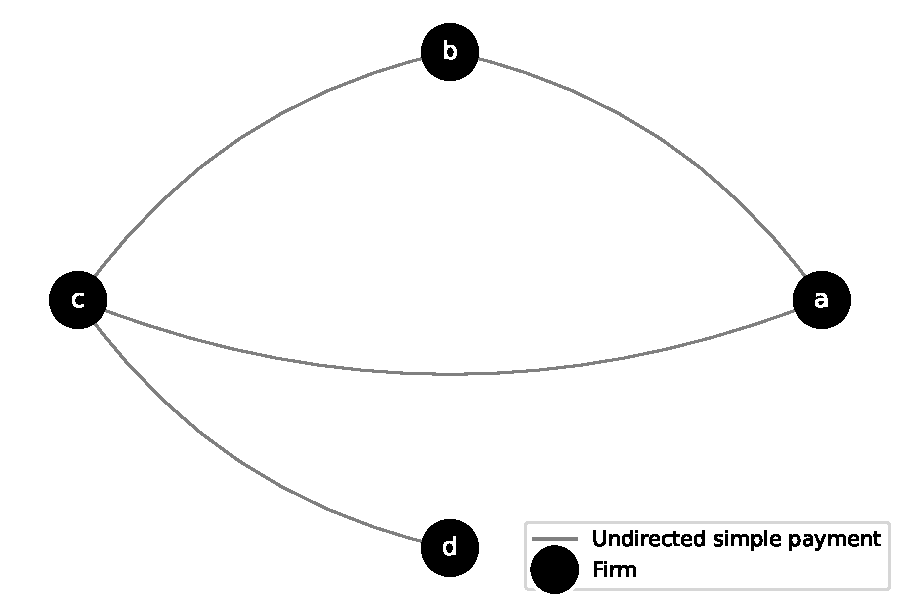
\includegraphics[width=8cm]{figures/F1.pdf}
 \captionof{figure}{\emph{Example 1} payment scenario}
 \vspace{0.5cm}
}
\end{mdframed}

Undirected simple payments represent the most primitive and simple payment transaction in this paper. As you might have noticed, the undirected payment, by definition,  does not contemplate multiple transactions (more than one transaction) payments between two parties and, therefore, firm $d$ in  \nameref{ex1} cannot have an additional payment transaction with firm $c$. 

To solve the multiple payment transaction limitation in the undirected simple payment, the general payment concept will be introduced and note it is a slightly extended version of the undirected simple payment.

\subsection{Undirected general payment} \label{ugp}
Undirected general payments in a market $G$ will be considered to be edges in a multigraph $G$ formed by a non-empty finite set $N(G)$ of nodes and a finite multiset $E(G)$ of unordered pairs of different elements of $N(G)$. The elements of $E(G)$ cannot contain identical pairs of $E(G)$, in other words,  self-loops are not allowed by definition in this payment method nor in any of the definitions proposed along all the paper. Note the \nameref{usp} differs from this payment definition because it does not allow multiple payment transactions between two firms as this payment method does.

\begin{mdframed}
\paragraph{Example 2} \label{ex2}
Let's imagine a payment scenario with four persons in which person $a$ is involved into two, parallel, payment transactions with person $b$, person $b$ with person $c$ and person $c$ with person $a$ and person $d$ in a market $G$. Then, $N(G) = \{a, b, c, d\}$ and $E(G) = \{ab, ab, bc, ca, cd\}$. Note $E(G) = \{ab, ab, bc, ca, cd\} = \{ba, ba, cb, ac, dc\}$ since $E(G)$ is unordered and therefore it does not specify the payer nor the payee.
\end{mdframed}

\subsection{Directed simple payment} \label{dsp}
Directed simple payments in a market $G$ will be considered to be arcs in a digraph $G$ made of a non-empty finite set $N(G)$ of nodes and a finite set $E(G)$ of distinct ordered pairs of distinct elements of $N(G)$, referred as arcs. Note $N(G)$ is the node set and $E(G)$ is the arc set and $G(N(G), E(G))$. The main difference with the undirected payments is that the directed payment specifies who is the payer and who the payee and that is why the pair elements of $E(G)$ are ordered.


\clearpage
\begin{mdframed}
\paragraph{Example 3} \label{ex3}
Let's imagine a payment scenario with four firms in which firm $a$ does a payment transaction to firm $b$, firm $b$ to firm $c$ and firm $c$ to firm $a$ and firm $d$ in a market $G$. Then, $N(G) = \{a, b, c, d\}$ and $E(G) = \{ab, bc, ca, cd\}$. Note $E(G) = \{ab, bc, ca, cd\} \neq \{bc, ab, cd, ca\}$ because the pair elements of $E(G)$ are ordered so now it is specified who is the payer and who the payee.
\end{mdframed}
% \clearpage
\subsection{Directed general payment} \label{dgp}
Directed general payments in a market $G$ will be considered to be arcs in a directed multigraph $G$ formed by a non-empty finite set $N(G)$ of nodes and a finite multiset $E(G)$ of ordered pairs of different elements of $N(G)$. The elements of $E(G)$, again, cannot contain identical pairs of $E(G)$. Note the \nameref{dsp} differs from this payment definition because it does not allow multiple payment transactions between two firms as this payment method does.

\begin{mdframed}
\paragraph{Example 4} \label{ex4}
Let's imagine a payment scenario with four persons in which person $a$ does a payment transaction to person $b$, $b$ to $a$, $b$ to $c$, $c$ to $b$, $c$ to $d$, $d$ to $a$ and $a$ to $d$ in a market $G$. Then, $N(G) = \{a, b, c, d\}$ and $E(G) = \{ab, ba, bc, cb, cd, dc, da, ad\}$.
{
 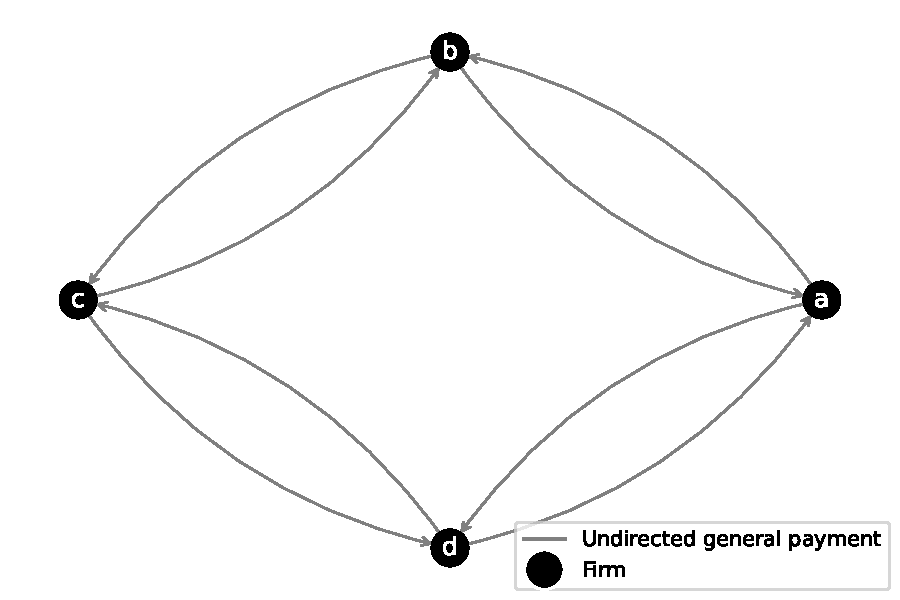
\includegraphics[width=8cm]{figures/F2.pdf}
 \captionof{figure}{\emph{Example 4} payment scenario}
 \vspace{0.5cm}
}
\end{mdframed}

\subsection{Payment quantification} \label{pq}
Summing up the different payments explained so far:

\begin{itemize}
  \item \nameref{usp} is a payment in which the payer and the payee are not defined and in which multilateral payments are not allowed.
  \item \nameref{ugp} is a payment in which the payer and the payee are not defined and in which multilateral payments are allowed.
  \item \nameref{dsp} is a payment in which the payer and the payee are defined and in which multilateral payments are not allowed.
  \item \nameref{dgp} is a payment in which the payer and the payee are defined and in which multilateral payments are allowed.
\end{itemize}

As we see the payments explained so far, do not specify in any way the amount to be paid nor the amount to be received by the payer and the payee respectively. To solve this problem the concepts of the \nameref{apm} and \nameref{upim} will be introduced to help labelling the graph, more specifically the payments, so the amount to be paid or received is quantified while keeping defined the payee and the payee. 

\subsubsection{Adjacency payment matrix} \label{apm}
The \nameref{apm} represents the relationship between firms with firms. It is nothing else than a $n \cdot n$ matrix $\textbf{A}$ where $n$ corresponds to the length and cardinality of the $N(G)$ set and equivalently to the amount of parties in the market $G$, so the $\textbf{A}_{ij}$ element of the matrix $\textbf{A}$ corresponds to the amount of payment transactions between the parties $i$ and $j$. So the element $\textbf{A}_{ij}$ will be $1$ if the party $i$ has issued or received a payment transaction from party $j$ and $0$ otherwise. Thus,

\begin{equation} \label{eq5}
\textbf{A}_{ij}(i, j) = \begin{cases}
			1, & \{i, j\} \in E\\
            0, & \text{otherwise}\\
		 \end{cases}
\end{equation}

Note that two parties $i$ and $j$ in a market $G$ will be considered to be adjacent if there exist at least one payment transaction $p$ between them and, in the same way, two payment transactions $x$ and $y$ in a market $G$ will be considered to be adjacent if there exist at least one party $z$ between the two payment transactions. 

In \nameref{ex1}, firm $c$ and $b$ are adjacent to each other because of the payment transaction $bc$ but also transactions $cb$ and $ba$ are adjacent to each other because of the firm $b$. 

% \clearpage
\begin{mdframed}
\paragraph{Example 5} \label{ex5}
The payment scenario of \nameref{ex1}, where  $N(G) = \{a, b, c, d\}$ and $E(G) = \{ab, bc, ca, cd\}$ in a market $G$ can be represented through an \nameref{apm} $\textbf{A}$ as follows:


\begin{equation} \label{eq6}
    \textbf{A} = \begin{blockarray}{ccccc}
 & a & b & c & d \\
\begin{block}{c[cccc]}
  a & 0 & 1 & 1 & 0 \\
  b & 1 & 0 & 1 & 0 \\
  c & 1 & 1 & 0 & 1 \\
  d & 0 & 0 & 1 & 0 \\
\end{block}
\end{blockarray}
\end{equation}

\emph{Note $\textbf{A}_{ij} \in \{0, 1\}, \forall i, j \in N$ where $\textbf{A}_{ij} = 0 \iff i = j, \forall i, j \in N$. Consequently, matrix $\textbf{A}$ diagonal are zeros (Hollow matrix), because self-payments are not allowed by definition. Note also that, the matrix  $\textbf{A}$ indicates how many transactions there are between the different parties of the market, but it does not quantify the payment and it does not specify the payers and payees of the market.}

\end{mdframed}

\subsubsection{Undirected payment incidence matrix} \label{upim}
The \nameref{upim} represents a relationship between firms with payments, rather than firms with firms as the \nameref{apm}. It is a payment incidence matrix but made of undirected payments, since the definition of the payment incidence matrix will be different for undirected payments and for directed ones, and therefore split, between the \nameref{upim} and the \nameref{dpim}.

An \nameref{upim} will be defined to be a $n \times m$ matrix $\textbf{I}$ where $n$ corresponds to the length and cardinality of the $N(G)$ set and equivalently to the amount of parties in a market of undirected payments $G$. Then, $m$ corresponds to the length and cardinality of the $E(G)$ set and equivalently to the amount of payment transactions in the market $G$, so if $i \in N$ and $\tau \in E$ the $\textbf{I}_{i\tau}$ element of the matrix $\textbf{I}$ corresponds to the relationship between the party $i$ and the payment transaction $\tau$ and . Thus,

\begin{equation} \label{eq:7}
 \textbf{I}_{i\tau} = \Phi(i, \tau) := \begin{cases}
			1, & i \in \tau\\
            0, & \text{otherwise}\\
		 \end{cases}
\end{equation}

\emph{Note $\Phi$ is the function, an indicator function, that gives the value of every element of the matrix and that it takes as input two sets, which correspond to the row and column of the matrix and then it outputs either 1 or 0, so $\Phi: (i, \tau) \rightarrow \{0, 1\}$}. 

% \clearpage
\begin{mdframed}
\paragraph{Example 6} \label{ex6}
The payment scenario of \nameref{ex1}, where  $N(G) = \{a, b, c, d\}$ and $E(G) = \{ab, bc, ca, cd\}$ in a market $G$ is actually a market scenario with undirected payments so $G$ can be represented through an \nameref{upim} $\textbf{I}$ as follows:


\begin{equation} \label{eq8}
    \textbf{I} = \begin{blockarray}{lcccc}
     & ab & bc & ca & cd  \\
\begin{block}{l[cccc]}
  a & 1 & 0 & 1 & 0  \\
  b & 1 & 1 & 0 & 0  \\
  c & 0 & 1 & 1 & 0  \\
  d & 0 & 0 & 0 & 1  \\
\end{block}
\end{blockarray}
\end{equation}

\emph{ Note $\textbf{I}_{ij} \in \{0, 1\}, \forall i \in N(G), \forall \tau \in E(G)$ and again the matrix does not quantify the payment nor specify the payers and payees of the market.}

\end{mdframed}

The \nameref{upim} has one important drawback, since its use is limited to the markets of undirected payments, it provides no more information, per se and in terms of quantitative market description, about the market transactions and parties than the \nameref{apm}. This is, in part, because the \nameref{upim} cannot provide additional market information that cannot be derived from the \nameref{apm} as stated in Proposition 1 and that is why the payment incidence matrix is separated when describing undirected payments and directed payments.

\paragraph{Proposition 1} In a connected market $G$ of \nameref{ugp}s, with $\eta$ firms and $\tau$ payment transactions, where $\eta \geq 2$ and $\tau \geq 1$, an \nameref{apm} $\textbf{A}$,  an \nameref{upim} $\textbf{I}$ and an identity matrix $\textbf{I}_{\tau}$ of size $\eta$, it is true that

\begin{equation} \label{9}
    \textbf{A}(\textbf{I}(G)) = (\textbf{I}(G)^{\top} \textbf{I}(G) - \tau \cdot \textbf{I}_{\eta})^{-}
\end{equation}

\subparagraph{Proof} Let $G$ denote a connected market with $\tau$ undirected payments with a set of parties $N$ and a multiset of payment transactions $E$. Let $\textbf{I}$ be the \nameref{upim}, $\textbf{A}$ the \nameref{apm} and $\textbf{L} = \textbf{I}^{\top} \textbf{I}$ of that market $G$. Then be $\Phi$ the function of equation \ref{eq:7}, $\textbf{L}_{ij}$ the $ij$-th element of the matrix $\textbf{L}$, $\textbf{A}_{ij}$ the $ij$-th of $\textbf{A}$ and $\textbf{I}_{ie}$ the $ie$-th of $\textbf{I}$. 

First, note that $\textbf{L}_{ij}$ is actually a function of $\Phi$:

\begin{equation} \label{eq10}
    \begin{split}
    & \textbf{L}_{ij} = \begin{blockarray}{cccc}
    \begin{block}{[cccc]}
    \textbf{I}_{i1} & \textbf{I}_{i2} & \cdots & \textbf{I}_{in} \\ \end{block}
    \end{blockarray}
    \begin{blockarray}{c}
    \begin{block}{[c]}
    \textbf{I}_{j1} \\
    \textbf{I}_{j2} \\
    \vdots \\
    \textbf{I}_{jn} \\
    \end{block}
    \end{blockarray} = \sum_{e \in E} \textbf{I}_{ie} \cdot \textbf{I}_{je} \\
    & = \sum_{e \in E} \Phi(i, e) \cdot \Phi(j, e) \\
    \end{split}
\end{equation}

Next, note that when $i = j$ then $\textbf{L}_{ij}$ is the degree of the party $i$, in other words, it equals the number of payment transactions in which party $i$ is involved, as shown in equation \ref{eq11}:

\begin{equation} \label{eq11}
    \begin{split}
        & i = j \implies \textbf{L}_{ij} = \sum_{e \in E} \Phi(i, e) \cdot \Phi(i, e) \\
        & = \sum_{e \in E} \Phi(i, e)^2 \\
    \end{split}
\end{equation}

On the other hand, when $i \neq j$ then the $ij$-th element of both matrices $\textbf{L}$ and $\textbf{A}$ are equal, as demonstrated in equation \ref{eq12}:

\begin{equation} \label{eq12}
    \begin{split}
        & i \neq j \implies \textbf{L}_{ij} = \sum_{e \in E} \Phi(i, e) \cdot \Phi(j, e) \\
        & = \sum_{e \in E} \Phi(ij, e) = \textbf{A}_{ij} \geq 0 \\
    \end{split}
\end{equation}

Consequently $\textbf{L}_{ij} = \textbf{A}_{ij}$ when $i \neq j$, so all non-diagonal elements of matrix $\textbf{L}$ will be equal to the non-diagonal elements of matrix $\textbf{A}$ and, subsequently, when we convert diagonal elements of matrix $\textbf{L}$ to $0$'s then  $\textbf{L} = \textbf{A}$ as demonstrated in equation \ref{eq13} and note it leads to Proposition 1. So, let $\textbf{I}_{\tau}$ be a identity matrix of size $\tau \times \tau$, then

\begin{equation} \label{eq13}
    \begin{split}
        & i = j \implies \textbf{L}_{ij} = \sum_{e \in E} \Phi(i, e)^2 \leq \sum_{e \in E} 1\\
        & \implies \textbf{L}_{ij} - \sum_{e \in E} 1 \leq 0 = \textbf{A}_{ij} \\
        & \implies (\textbf{L} - (\sum_{e \in  E} 1) \cdot \textbf{I}_{\eta})^{-} = \textbf{A}\\
        & \therefore i = j \lor i \neq j \implies (\textbf{I}^{\top}\textbf{I} - \tau \cdot \textbf{I}_{\tau})^{-} = \textbf{A} \\
        & \implies \textbf{A}(\textbf{I}(G)) = (\textbf{I}(G)^{\top}\textbf{I}(G) - \tau \cdot \textbf{I}_{\tau})^{-} \\
    \end{split}
\end{equation}

\emph{As a matter of curiosity, $\textbf{L}$, which is also known as a Laplacian matrix, could have been used as a substitute for convenience purposes of the \nameref{upim} but since it is easily derivable it will not be used.}

The \nameref{upim} describing a market of undirected payments is a function of the \nameref{apm} and no more useful than it, but the use of a payment incidence matrix to represent directed payments gives additional and more important information in comparison with the undirected ones and that's why the \nameref{dpim} concept will be introduced.

\subsubsection{Directed payment incidence matrix} \label{dpim}

The \nameref{dpim}, an extension of the \nameref{upim}, is an incidence matrix limited to the use in a market of directed payments. It is nothing else than a $n \times m$ matrix $\textbf{I}$ where $n$ corresponds to the length and cardinality of the $N(G)$ set and equivalently to the amount of parties in a market of directed payments $G$. Then, $m$ corresponds to the length and cardinality of the $E(G)$ multiset and equivalently to the amount of payment transactions in the market $G$, so if $i \in N$ and $\tau \in E$ the $\textbf{I}_{i\tau}$ element of the matrix $\textbf{I}$ corresponds not to the relationship, but to the amount of relationships, between the party $i$ and the directed payment transaction $\tau$ or alternatively to the amount of transactions $\tau$ associated with party $i$. Let $\Phi$ be the function of equation \ref{eq:7}, then

\begin{equation}
\textbf{I}_{i\tau} = \Theta(i, \tau) := \sum_{e \in E} \Phi (\tau, E)
\end{equation}

\emph{Note $\Theta$, a function that gives you the value of each specific element of the matrix $\mathbf{I}$,  maps two sets into a positive integer or 0, so $\Theta: (i, \tau) \rightarrow \mathbb{Z}^{0+}$}.

% \clearpage
\begin{mdframed}
\paragraph{Example 7} \label{ex7}
The payment scenario of \nameref{ex4} where  $N(G) = \{a, b, c, d\}$ and $E(G) = \{ab, ba, bc, cb, cd, dc, da, ad\}$ in a market $G$ is actually a market scenario with directed payments so $G$ can be represented through a \nameref{dpim} $\textbf{I}$ as follows:


\begin{equation} \label{eq8}
    \textbf{I} = \begin{blockarray}{lcccccccc}
     & ab & ba & bc & cb & cd & dc & da & ad \\
\begin{block}{l[cccccccc]}
  a & 1 & 1 & 0 & 0 & 0 & 0 & 1 & 1 \\
  b & 1 & 1 & 1 & 1 & 0 & 0 & 0 & 0 \\
  c & 0 & 0 & 1 & 1 & 1 & 1 & 0 & 0 \\
  d & 0 & 0 & 0 & 0 & 1 & 1 & 1 & 1 \\
\end{block}
\end{blockarray}
\end{equation}

\emph{ Note that even though $\textbf{I}_{i\tau} \in \mathbb{Z}^{0+}, \forall i \in N(G), \forall \tau \in E(G)$, all the elements are $1$'s or $0$'s because there are not repeated payments, since if there were two $ab$ payments in the market then $\textbf{I}_{a \text{ }ab}, \textbf{I}_{b \text{ }ab}$ = 2}.

\end{mdframed}

Finally and to summarize:

\begin{itemize}
  \item \nameref{apm} can be used to describe a market of either \nameref{usp}s or \nameref{ugp}s.
  \item \nameref{upim} can also be used to describe a market of either \nameref{usp}s, \nameref{ugp}s with the respective differences explained in their sections.
  \item \nameref{dpim} can be used to describe a market of either.
\end{itemize}.



\subsection{Directed net payment} \label{dnp}
\nameref{dnp}s will be considered to be payments in a market $G$ where a \nameref{dgp} are multilaterally set-off so each payment can take a \nameref{dsp} form. These directed net payments will be considered to be arcs in a directed simple graph $G$ formed by a non-empty finite set $N(G)$ of nodes and a finite set $E(G)$ of ordered pairs of different elements of $N(G)$.

\subsection{Submarket}
A market $G$ will be considered to have a submarket $G^{\prime}$ if the submarket expressed as a graph is a subgraph of the market $G$ expressed as a graph. Then the market $G^{\prime}$ will be a submarket of $G$ if the set of firms and payment transactions are subsets of the set of firms and payment transactions of the market $G$ and therefore $G^{\prime} \subset G \iff (N(G^{\prime}) \subset N(G)) \land(E(G^{\prime}) \subset E(G))$.


\cite{wilson1979introduction}
\cite{lisbonne2020blockchainmath}
\section{Acknowledgements}
This work was supervised the Dr. Alexandra Simon Villar, who helped me in many different aspects along the project.
\printbibliography %Prints bibliography
\end{multicols}
\end{document}

